% !TeX program = pdflatex
% Standalone Beamer source; all diagrams are drawn in LaTeX.
% Standalone Beamer source; all diagrams are drawn in LaTeX.
% Standalone Beamer source; all diagrams are drawn in LaTeX.
\documentclass[aspectratio=169,11pt]{beamer}
\usetheme{Singapore}
\usecolortheme{default}
\usefonttheme{default}
\usepackage[T1]{fontenc}
\usepackage[utf8]{inputenc}
\usepackage[english]{babel}
\usepackage{textcomp,lmodern,amsmath,amssymb,mathtools,booktabs}
\usepackage{tikz,pgfplots,adjustbox}
\usetikzlibrary{arrows.meta,positioning,calc,matrix,fit,backgrounds}
\pgfplotsset{compat=1.18}
\definecolor{BG}{HTML}{FFFFFF}
\definecolor{Panel}{HTML}{F5F5F5}
\definecolor{Ink}{HTML}{202020}
\definecolor{Muted}{HTML}{555555}
\definecolor{Weight}{HTML}{244A85}
\definecolor{Data}{HTML}{9B5100}
\definecolor{Vec}{HTML}{266449}
\definecolor{Prob}{HTML}{A12B35}
% Standalone Beamer source; all diagrams are drawn in LaTeX.
\setbeamertemplate{navigation symbols}{}
\setbeamerfont{frametitle}{size=\large}
\setbeamerfont{normal text}{size=\small}
\AtBeginEnvironment{frame}{\small}
\setlength{\emergencystretch}{1em}
\setbeamertemplate{footline}[frame number]
\setbeamertemplate{bibliography item}[text]
\setbeamertemplate{section in toc}[sections numbered]
\setbeamerfont{section in toc}{size=\small}
\setbeamersize{text margin left=8mm,text margin right=8mm}
\setlength{\abovedisplayskip}{5pt}
\setlength{\belowdisplayskip}{5pt}
\hypersetup{colorlinks=true,urlcolor=Weight,linkcolor=Ink}
\newcommand{\w}[1]{{\color{Weight}#1}}
\newcommand{\dat}[1]{{\color{Data}#1}}
\newcommand{\vv}[1]{{\color{Vec}#1}}
\newcommand{\pr}[1]{{\color{Prob}#1}}
\newcommand{\msg}[1]{\par\medskip{\small\textbf{Key idea:} #1\par}}
\newcommand{\src}[1]{\par\vspace{1mm}{\scriptsize\color{Muted}#1\par}}
\newcommand{\R}{\mathbb{R}}
\tikzset{
  >={Latex[length=2.2mm]},
  box/.style={draw=Muted!45,fill=white,
    minimum height=9mm,align=center,inner sep=6pt,font=\small},
  input/.style={box,draw=Data,text=Data},
  param/.style={box,draw=Weight,text=Weight},
  vector/.style={box,draw=Vec,text=Vec},
  output/.style={box,draw=Prob,text=Prob},
  flow/.style={->,line width=1pt,draw=Muted},
  axis/.style={->,draw=Muted!80,line width=.6pt},
  gridline/.style={draw=Muted!18,line width=.3pt},
  vflow/.style={->,draw=Vec,line width=1.1pt},
  tinylabel/.style={font=\scriptsize,text=Muted}
}
\pgfplotsset{deck/.style={
  axis background/.style={fill=BG},axis line style={Muted},
  tick style={Muted},tick label style={font=\scriptsize,color=Muted},
  label style={font=\small,color=Ink},title style={font=\small,color=Ink},
  grid style={Muted!15},every axis plot/.append style={line width=.9pt}}}
% Standalone Beamer source; all diagrams are drawn in LaTeX.
\newcommand{\bars}[4]{%
\begin{adjustbox}{max width=\linewidth,max totalheight=4.2cm}
\begin{tikzpicture}
\begin{axis}[deck,width=4.1cm,height=3.25cm,ybar,bar width=17pt,
 ymin=0,ymax=105,ytick={0,50,100},yticklabels={0,50,100},
 xmin=.4,xmax=3.6,xtick={1,2,3},xticklabels={blue,cloudy,sunny},
 x tick label style={font=\tiny,rotate=20,anchor=east},
 title={#1},ylabel={\%},axis lines*=left,ymajorgrids,
 nodes near coords,nodes near coords style={font=\tiny,color=Prob},
 point meta=y]
\addplot[fill=Prob!65,draw=Prob] coordinates {(1,#2)(2,#3)(3,#4)};
\end{axis}
\end{tikzpicture}
\end{adjustbox}}
\title[Transformers and LLMs]{Transformers and Large Language Models}
\subtitle{Mathematical foundations and model architecture}
\author{}
\institute{}
\date{}
\begin{document}

% 01 ---------------------------------------------------------------
\begin{frame}[plain]
\titlepage
\end{frame}

\begin{frame}{Contents}
\begin{columns}[T,onlytextwidth]
\column{.48\textwidth}
\tableofcontents[sections={1-5}]
\column{.48\textwidth}
\tableofcontents[sections={6-11}]
\end{columns}
\end{frame}
\section[GPT]{Introduction}

% 02 ---------------------------------------------------------------
\begin{frame}[fragile]{GPT: three terms, one model family}
\begin{columns}[T,onlytextwidth]
\column{.53\textwidth}
\textbf{Large Language Model (LLM):} a large neural language model that
learns statistical patterns in text.
\medskip
\begin{adjustbox}{max width=\linewidth,max totalheight=4.2cm}
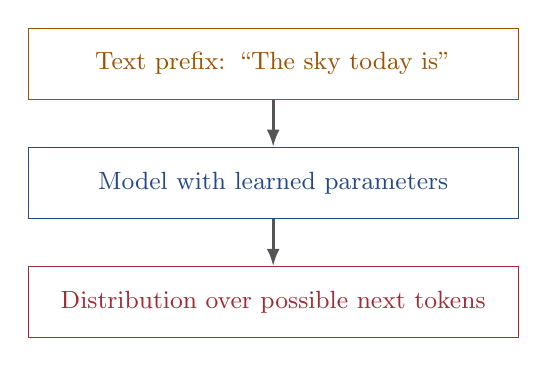
\begin{tikzpicture}
\node[input,text width=5.8cm] (a) {Text prefix: ``The sky today is''};
\node[param,text width=5.8cm,below=6mm of a] (b) {Model with learned parameters};
\node[output,text width=5.8cm,below=6mm of b] (c) {Distribution over possible next tokens};
\draw[flow] (a)--(b);\draw[flow] (b)--(c);
\end{tikzpicture}
\end{adjustbox}
\column{.43\textwidth}
\textcolor{Data}{\Large G}\enspace\textbf{Generative}\\
Produces new token sequences.
\medskip

\textcolor{Weight}{\Large P}\enspace\textbf{Pretrained}\\
Initially learns from many training examples.
\medskip

\textcolor{Vec}{\Large T}\enspace\textbf{Transformer}\\
A network architecture that processes representations in context.
\end{columns}
\msg{Here we study \textbf{autoregressive GPT language models}: They generate one token at a time.}
\src{\cite{sanderson2024} Not every LLM is a GPT. Chat assistants may undergo additional post-training.}
\end{frame}

% 03 ---------------------------------------------------------------
\begin{frame}[fragile]{Text generation through repeated prediction}
\centering
\begin{adjustbox}{max width=\linewidth,max totalheight=4.2cm}
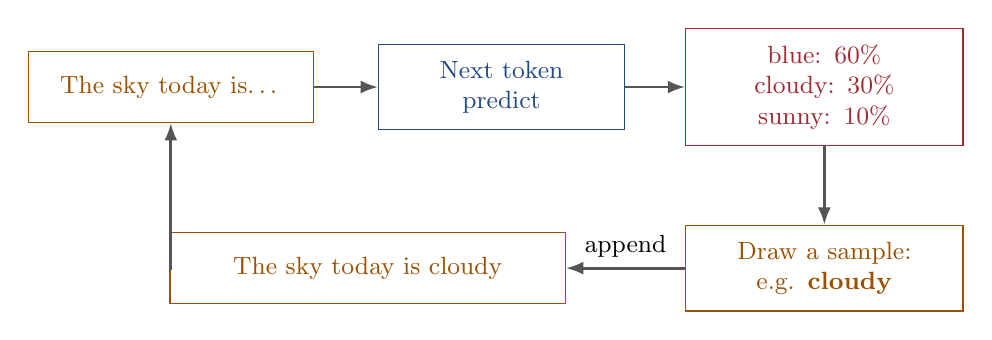
\begin{tikzpicture}
\node[input,text width=3.2cm] (a) at (0,0) {The sky today is\ldots};
\node[param,text width=2.7cm] (b) at (4.2,0) {Next token\\predict};
\node[output,text width=3.1cm] (c) at (8.3,0) {blue: 60\%\\cloudy: 30\%\\sunny: 10\%};
\node[input,text width=3.1cm] (d) at (8.3,-2.3) {Draw a sample:\\e.g. \textbf{cloudy}};
\node[input,text width=4.6cm] (e) at (2.5,-2.3) {The sky today is cloudy};
\draw[flow] (a)--(b);\draw[flow] (b)--(c);\draw[flow] (c)--(d);
\draw[flow] (d)--node[above,font=\small]{append}(e);
\draw[flow] (e.west)-| (a.south);
\end{tikzpicture}
\end{adjustbox}
\msg{\textbf{Sampling} selects a token at random according to the probabilities. The second most likely token can also be selected.}
\raggedright
\src{\cite{sanderson2024} Constructed three-token vocabulary; real models assign probability to many more tokens.\\
Autoregressive: earlier tokens become input for the next step. Stop at an end token or a length limit.}
\end{frame}

% 04 ---------------------------------------------------------------
\section[Learning]{Learning and parameters}
\begin{frame}[fragile]{Machine learning starts with adjustable parameters}
\begin{columns}[T,onlytextwidth]
\column{.47\textwidth}
\textbf{Machine Learning:} Learn behaviour from data rather than specifying every rule.
\[
\hat y=\w{m}\dat{x}+\w{b}
\]
\textbf{Linear regression:} fit a straight line to data.
\medskip

\dat{$x$}: Input; $\hat y$: Prediction.\\
\w{$m$}: slope; \w{$b$}: intercept.
\[
\begin{gathered}
\dat{x=2},\quad\w{m=2,\ b=1}\\
\Rightarrow\quad\pr{\hat y=5}
\end{gathered}
\]
\column{.50\textwidth}
\begin{adjustbox}{max width=\linewidth,max totalheight=4.2cm}
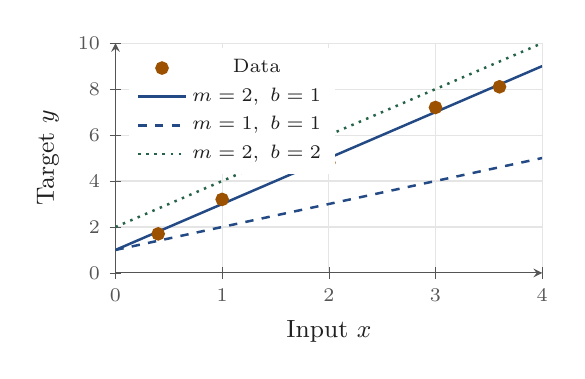
\begin{tikzpicture}
\begin{axis}[deck,width=7cm,height=4.5cm,xmin=0,xmax=4,ymin=0,ymax=10,
 xlabel={Input $x$},ylabel={Target $y$},grid=major,axis lines=left,
 legend style={draw=none,fill=BG,text=Ink,font=\scriptsize,at={(.03,.98)},anchor=north west}]
\addplot[only marks,mark=*,Data] coordinates {(.4,1.7)(1,3.2)(2,4.8)(3,7.2)(3.6,8.1)};
\addlegendentry{Data}
\addplot[Weight,domain=0:4]{2*x+1};\addlegendentry{$m=2,\ b=1$}
\addplot[Weight,dashed,domain=0:4]{x+1};\addlegendentry{$m=1,\ b=1$}
\addplot[Vec,dotted,domain=0:4]{2*x+2};\addlegendentry{$m=2,\ b=2$}
\end{axis}
\end{tikzpicture}
\end{adjustbox}
\end{columns}
\msg{A \textbf{parameter} is a learned adjustable value: changing it changes the predictions.}
\src{\cite{sanderson2024} Supplementary linear regression example. All data points are constructed.}
\end{frame}

% 05 ---------------------------------------------------------------
\begin{frame}[fragile]{Training: measure errors and adjust weights}
\centering
\begin{adjustbox}{max width=\linewidth,max totalheight=4.2cm}
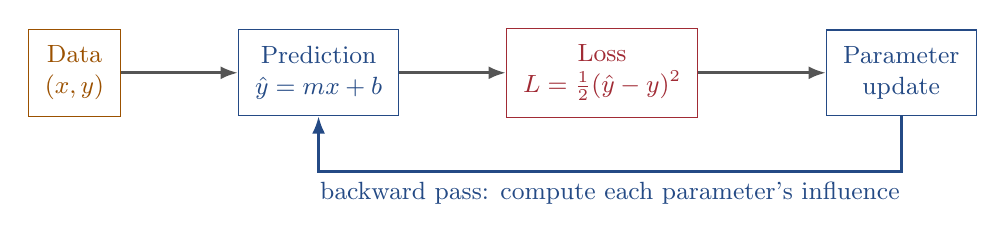
\begin{tikzpicture}
\node[input] (a) at (0,0) {Data\\$(x,y)$};
\node[param] (b) at (3.1,0) {Prediction\\$\hat y=mx+b$};
\node[output] (c) at (6.7,0) {Loss\\$L=\frac12(\hat y-y)^2$};
\node[param] (d) at (10.5,0) {Parameter\\update};
\draw[flow] (a)--(b);\draw[flow] (b)--(c);\draw[flow] (c)--(d);
\draw[flow,Weight] (d.south)--++(0,-.7)-|node[pos=.25,below,font=\small]{backward pass: compute each parameter's influence}(b.south);
\end{tikzpicture}
\end{adjustbox}
\vspace{3mm}
\begin{columns}[T,onlytextwidth]
\column{.49\textwidth}
\textbf{Backpropagation} computes derivatives using the chain rule.\\[2mm]
A \textbf{gradient} describes how the loss changes when parameters change.
\column{.48\textwidth}
\small
One data point: $x=2,\ y=5$; Initial values: $m=1,b=0$.\\
$\hat y=2$, error $\hat y-y=-3$, $L=4.5$.
\[
\begin{aligned}
\frac{\partial L}{\partial m}&=-3\cdot2=-6,\\
\frac{\partial L}{\partial b}&=-3
\end{aligned}
\]
\textbf{Gradient descent}, learning rate $\eta=0.1$:\\
$m'=1-0.1(-6)=1.6$, $b'=0.3$.\\
New prediction: $3.5$; new loss: $L'=1.125$.
\end{columns}
\end{frame}

% 06 ---------------------------------------------------------------
\begin{frame}[fragile]{Neural networks combine simple computations}
\begin{columns}[T,onlytextwidth]
\column{.51\textwidth}
\begin{adjustbox}{max width=\linewidth,max totalheight=4.2cm}
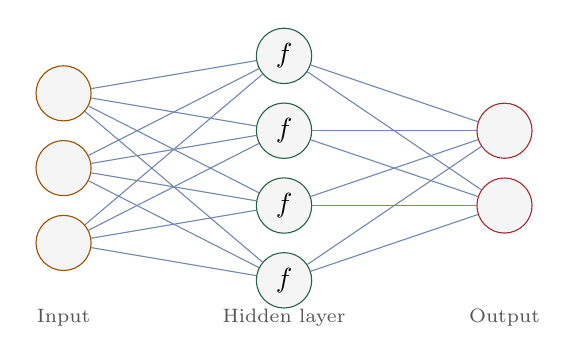
\begin{tikzpicture}[x=1.4cm,y=.95cm]
\foreach \i in {1,2,3} \node[circle,draw=Data,fill=Panel,minimum size=7mm] (i\i) at (0,\i) {};
\foreach \i in {1,2,3,4} \node[circle,draw=Vec,fill=Panel,minimum size=7mm] (h\i) at (2,\i-.5) {$f$};
\foreach \i in {1,2} \node[circle,draw=Prob,fill=Panel,minimum size=7mm] (o\i) at (4,\i+.5) {};
\foreach \i in {1,2,3} \foreach \j in {1,2,3,4} \draw[Weight!65] (i\i)--(h\j);
\foreach \i in {1,2,3,4} \foreach \j in {1,2} \draw[Weight!65] (h\i)--(o\j);
\node[tinylabel] at (0,0) {Input};\node[tinylabel] at (2,0) {Hidden layer};
\node[tinylabel] at (4,0) {Output};
\end{tikzpicture}
\end{adjustbox}
\[
\vv{h_j}=f\!\left(\sum_i\w{w_{ji}}\dat{x_i}+\w{b_j}\right)
\]
\column{.45\textwidth}
\textbf{Weights} scale contributions. A \textbf{Bias} shifts the sum.\\[2mm]
An \textbf{activation function} $f$ introduces a nonlinear transformation, e.g. $f(s)=\max(0,s)$.
\medskip

Without nonlinearity, several affine layers would still compose to \textbf{one affine map}.
\medskip

More parameters increase capacity, but do not guarantee quality. Data, architecture and training must work together.
\end{columns}
\src{Supplement: Overfitting means fitting training data while generalizing poorly to new data.}
\end{frame}

% 07 ---------------------------------------------------------------
\section[Math]{Numbers and geometry}
\begin{frame}[fragile]{Scalars, vectors and matrices are tensors}
\centering
\begin{adjustbox}{max width=\linewidth,max totalheight=4.2cm}
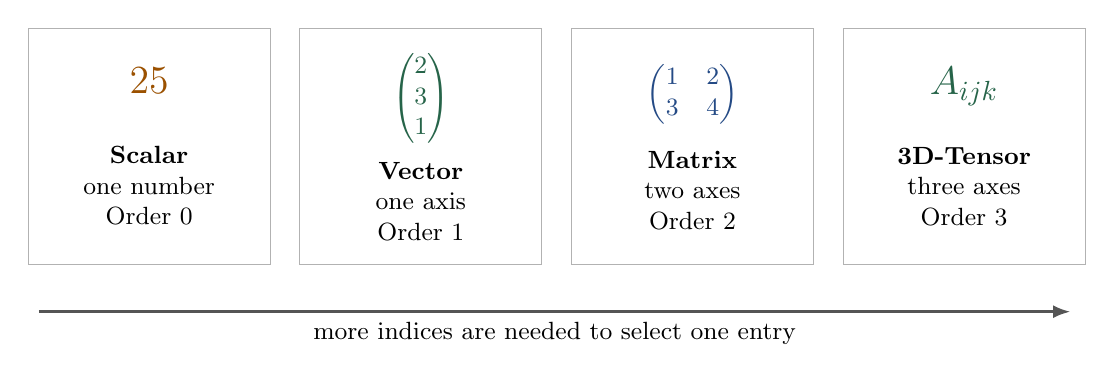
\begin{tikzpicture}
\node[box,text width=2.65cm,minimum height=3.0cm] at (0,0)
 {\textcolor{Data}{\Large $25$}\\[5mm]\textbf{Scalar}\\one number\\Order 0};
\node[box,text width=2.65cm,minimum height=3.0cm] at (3.45,0)
 {\textcolor{Vec}{$\begin{pmatrix}2\\3\\1\end{pmatrix}$}\\[2mm]\textbf{Vector}\\one axis\\Order 1};
\node[box,text width=2.65cm,minimum height=3.0cm] at (6.9,0)
 {\textcolor{Weight}{$\begin{pmatrix}1&2\\3&4\end{pmatrix}$}\\[3mm]\textbf{Matrix}\\two axes\\Order 2};
\node[box,text width=2.65cm,minimum height=3.0cm] at (10.35,0)
 {\textcolor{Vec}{\Large $A_{ijk}$}\\[5mm]\textbf{3D-Tensor}\\three axes\\Order 3};
\draw[flow] (-1.4,-2.1)--node[below,font=\small]{more indices are needed to select one entry}(11.7,-2.1);
\end{tikzpicture}
\end{adjustbox}
\msg{In deep learning, a \textbf{tensor} is a numerical array. Its order counts the axes; its \textbf{shape} gives their lengths.}
\src{Supplement: tensor rank here means the number of axes, not matrix rank or algebraic tensor rank.\\
A vector with 3 components has shape $(3)$ and order 1.}
\end{frame}

% 08 ---------------------------------------------------------------
\begin{frame}[fragile]{A vector is a list, a point and an arrow}
\begin{columns}[T,onlytextwidth]
\column{.52\textwidth}
\centering
\begin{adjustbox}{max width=\linewidth,max totalheight=4.2cm}
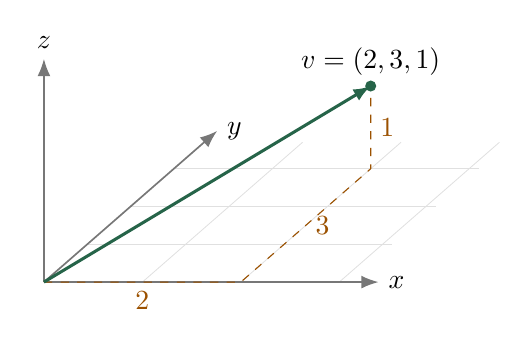
\begin{tikzpicture}[x={(1.25cm,0cm)},y={(.55cm,.48cm)},z={(0cm,1.05cm)}]
\foreach \i in {0,1,2,3} {
 \draw[gridline] (\i,0,0)--(\i,3.7,0);
 \draw[gridline] (0,\i,0)--(3.1,\i,0);}
\draw[axis] (0,0,0)--(3.4,0,0) node[right]{$x$};
\draw[axis] (0,0,0)--(0,4,0) node[right]{$y$};
\draw[axis] (0,0,0)--(0,0,2.7) node[above]{$z$};
\draw[Data,dashed] (0,0,0)--(2,0,0)--(2,3,0)--(2,3,1);
\node[below,Data] at (1,0,0) {$2$};
\node[right,Data] at (2,1.5,0) {$3$};
\node[right,Data] at (2,3,.5) {$1$};
\draw[vflow] (0,0,0)--(2,3,1) node[above]{$v=(2,3,1)$};
\fill[Vec] (2,3,1) circle (2pt);
\end{tikzpicture}
\end{adjustbox}
\column{.44\textwidth}
\[
\vv{v}=\begin{pmatrix}2\\3\\1\end{pmatrix}\in\R^3
\]
\textbf{Components}: steps along the three axes.\\[2mm]
\textbf{Direction}: from the origin to the point.\\[2mm]
\textbf{Length} (Euclidean norm):
\[
\begin{aligned}
\|v\|&=\sqrt{2^2+3^2+1^2}\\
&=\sqrt{14}\approx3.74.
\end{aligned}
\]
\end{columns}
\msg{The three numbers specify a position; the same vector can be drawn as an arrow from the origin.}
\end{frame}

% 09 ---------------------------------------------------------------
\begin{frame}[fragile]{Vector addition: join arrows head to tail}
\begin{columns}[T,onlytextwidth]
\column{.49\textwidth}
\centering\textbf{Addition}
\[
\vv{\begin{pmatrix}2\\1\end{pmatrix}}+
\dat{\begin{pmatrix}1\\2\end{pmatrix}}=
\pr{\begin{pmatrix}3\\3\end{pmatrix}}
\]
\begin{adjustbox}{max width=\linewidth,max totalheight=4.2cm}
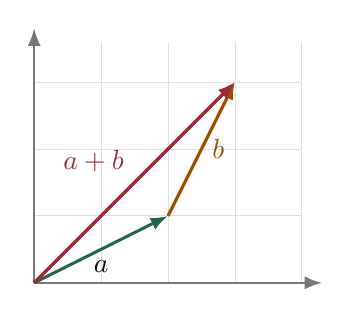
\begin{tikzpicture}[scale=.85]
\draw[gridline,step=1] (0,0) grid (4,3.6);
\draw[axis] (0,0)--(4.3,0);\draw[axis] (0,0)--(0,3.8);
\draw[vflow] (0,0)--(2,1) node[midway,below]{$a$};
\draw[->,Data,very thick] (2,1)--(3,3) node[midway,right]{$b$};
\draw[->,Prob,very thick] (0,0)--(3,3) node[midway,above left]{$a+b$};
\end{tikzpicture}
\end{adjustbox}
\column{.48\textwidth}
\centering\textbf{Scaling}
\[
2\vv{\begin{pmatrix}2\\1\end{pmatrix}}=
\vv{\begin{pmatrix}4\\2\end{pmatrix}}
\]
\begin{adjustbox}{max width=\linewidth,max totalheight=4.2cm}
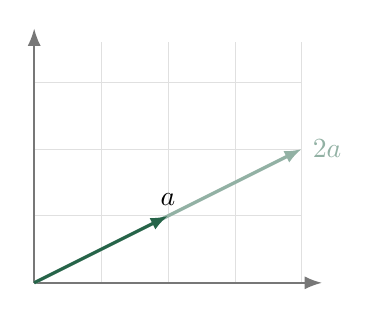
\begin{tikzpicture}[scale=.85]
\draw[gridline,step=1] (0,0) grid (4,3.6);
\draw[axis] (0,0)--(4.3,0);\draw[axis] (0,0)--(0,3.8);
\draw[->,Vec!50,very thick] (0,0)--(4,2) node[right]{$2a$};
\draw[vflow] (0,0)--(2,1) node[above]{$a$};
\end{tikzpicture}
\end{adjustbox}
\end{columns}
\msg{Addition works component by component. A positive factor changes the length; a negative factor reverses the direction.}
\end{frame}

% 10 ---------------------------------------------------------------
\begin{frame}[fragile]{A matrix combines multiple weighted sums}
\begin{columns}[T,onlytextwidth]
\column{.44\textwidth}
\centering
\begin{adjustbox}{max width=\linewidth,max totalheight=4.2cm}
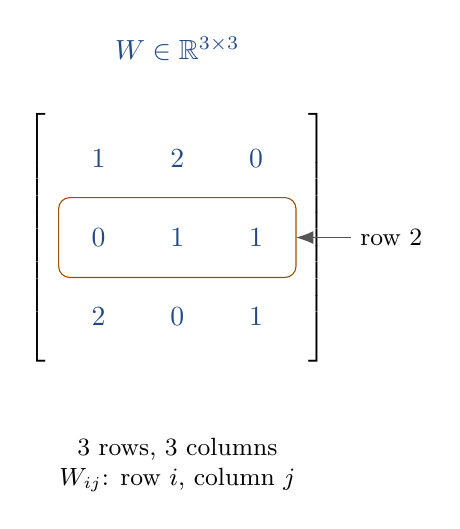
\begin{tikzpicture}
\matrix (m) [matrix of math nodes,nodes={minimum width=10mm,minimum height=10mm,text=Weight},
 left delimiter={[},right delimiter={]}] {1&2&0\\0&1&1\\2&0&1\\};
\node[above=5mm of m,text=Weight] {$W\in\R^{3\times3}$};
\draw[Data,rounded corners] (m-2-1.north west) rectangle (m-2-3.south east);
\node[below=8mm of m,align=center,font=\small] {3 rows, 3 columns\\$W_{ij}$: row $i$, column $j$};
\draw[->,Muted] (2.2,.0)--(m-2-3.east);
\node[right,font=\small] at (2.2,0) {row 2};
\end{tikzpicture}
\end{adjustbox}
\column{.52\textwidth}
\textbf{Matrix-vector product:} Each row produces one output component.
\[
\vv{y_i}=\sum_{j=1}^3\w{W_{ij}}\dat{x_j}
\]
\begin{adjustbox}{max width=\linewidth,max totalheight=4.2cm}
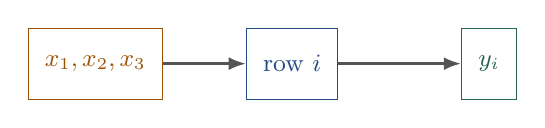
\begin{tikzpicture}
\node[input] (x) at (0,0) {$x_1,x_2,x_3$};
\node[param] (w) at (2.5,0) {row $i$};
\node[vector] (y) at (5,0) {$y_i$};
\draw[flow] (x)--(w);\draw[flow] (w)--(y);
\end{tikzpicture}
\end{adjustbox}
\medskip

An $m\times n$ matrix maps $n$ input components to $m$ output components.
\end{columns}
\msg{The number of columns of $W$ must match the length of $x$: $(m\times n)(n\times1)=(m\times1)$.}
\src{Supplement: throughout this presentation, vectors are column vectors.}
\end{frame}

% 11 ---------------------------------------------------------------
\begin{frame}[fragile]{A matrix product, step by step}
\[
\underbrace{\vv{\begin{pmatrix}8\\4\\5\end{pmatrix}}}_{\text{Output }y}
=\underbrace{\w{\begin{pmatrix}1&2&0\\0&1&1\\2&0&1\end{pmatrix}}}_{\text{Weights }W}
\underbrace{\dat{\begin{pmatrix}2\\3\\1\end{pmatrix}}}_{\text{Input }x}
\]
\vspace{2mm}
\begin{columns}[T,onlytextwidth]
\column{.52\textwidth}
\begin{align*}
y_1&=\w1\cdot\dat2+\w2\cdot\dat3+\w0\cdot\dat1=\vv8,\\
y_2&=\w0\cdot\dat2+\w1\cdot\dat3+\w1\cdot\dat1=\vv4,\\
y_3&=\w2\cdot\dat2+\w0\cdot\dat3+\w1\cdot\dat1=\vv5.
\end{align*}
\column{.44\textwidth}
\centering
\begin{adjustbox}{max width=\linewidth,max totalheight=4.2cm}
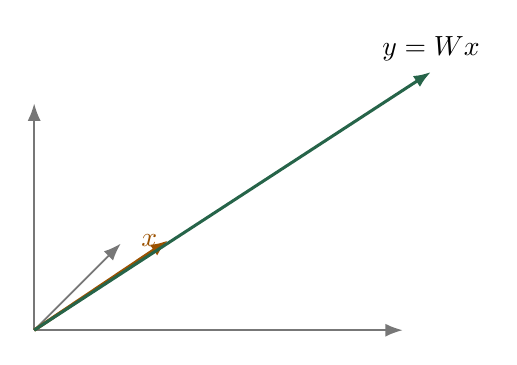
\begin{tikzpicture}[x={(.52cm,0cm)},y={(.22cm,.22cm)},z={(0cm,.48cm)}]
\draw[axis] (0,0,0)--(9,0,0);\draw[axis] (0,0,0)--(0,5,0);\draw[axis] (0,0,0)--(0,0,6);
\draw[->,Data,very thick] (0,0,0)--(2,3,1) node[left]{$x$};
\draw[vflow] (0,0,0)--(8,4,5) node[above]{$y=Wx$};
\end{tikzpicture}
\end{adjustbox}
\end{columns}
\msg{The same calculation can be understood as \textbf{weighted sums} or as a \textbf{geometric transformation}.}
\end{frame}

% 12 ---------------------------------------------------------------
\begin{frame}[fragile]{A tensor adds further axes to a numerical array}
\begin{columns}[T,onlytextwidth]
\column{.50\textwidth}
\centering
\begin{adjustbox}{max width=\linewidth,max totalheight=4.2cm}
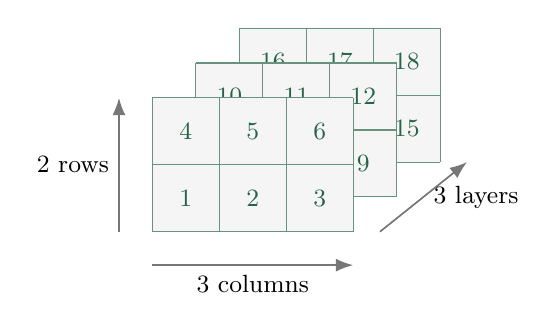
\begin{tikzpicture}[scale=.85]
\foreach \k in {2,1,0} {
 \begin{scope}[shift={(\k*.65,\k*.52)}]
 \fill[Panel] (0,0) rectangle (3,2);
 \draw[Vec!70] (0,0) grid[step=1] (3,2);
 \foreach \x in {0,1,2} \foreach \y in {0,1} {
  \pgfmathtruncatemacro{\val}{1+\x+3*\y+6*\k}
  \node[text=Vec,font=\small] at (\x+.5,\y+.5) {\val};}
 \end{scope}}
\draw[axis] (0,-.5)--node[below,font=\small]{3 columns}(3,-.5);
\draw[axis] (-.5,0)--node[left,font=\small]{2 rows}(-.5,2);
\draw[axis] (3.4,0)--node[right,font=\small]{3 layers}(4.7,1.04);
\end{tikzpicture}
\end{adjustbox}
\column{.46\textwidth}
\textbf{Three indices} select one entry:
\[
A_{ijk},\qquad\text{Shape }(2,3,3).
\]
The block contains $2\cdot3\cdot3=18$ numbers.
\medskip

\textbf{In a language model:}
\[
\underbrace{B}_{\text{texts}}\times
\underbrace{n}_{\text{Tokens}}\times
\underbrace{d}_{\text{features}}
\]
A \textbf{batch} groups $B$ examples. Each text has $n$ token vectors of length $d$.
\end{columns}
\msg{A tensor axis need not represent a spatial direction: it can index texts or token positions.}
\src{Supplement: below, we consider one text and arrange its token vectors as columns in $\R^{d\times n}$.}
\end{frame}

% 13 ---------------------------------------------------------------
\section[Tokens]{Tokenization and embeddings}
\begin{frame}[fragile]{Tokenization: split text into addressable units}
\centering
\textcolor{Data}{\Large ChatGPT understands language.}\par\vspace{3mm}
\begin{adjustbox}{max width=\linewidth,max totalheight=4.2cm}
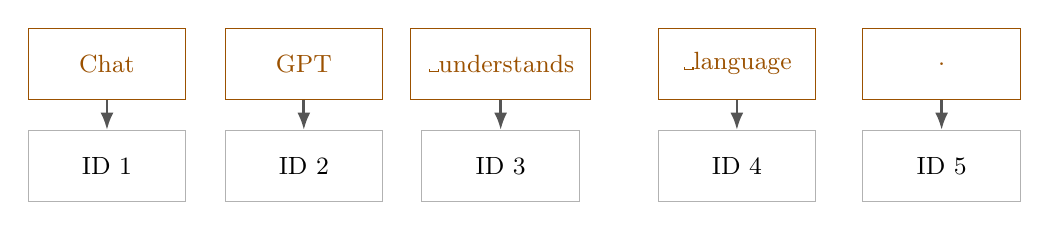
\begin{tikzpicture}
\foreach \x/\s/\id in {0/Chat/1,2.5/GPT/2,5/{\textvisiblespace understands}/3,8/{\textvisiblespace language}/4,10.6/./5} {
 \node[input,minimum width=2cm] (t\id) at (\x,0) {\s};
 \node[box,minimum width=2cm] (i\id) at (\x,-1.3) {ID \id};
 \draw[flow] (t\id)--(i\id);}
\end{tikzpicture}
\end{adjustbox}
\vspace{5mm}
\begin{columns}[T,onlytextwidth]
\column{.48\textwidth}
A \textbf{token} can be a word, a word fragment, punctuation or another text unit.
\column{.48\textwidth}
The \textbf{vocabulary} is the fixed list of possible tokens. Each token has a unique \textbf{ID}.
\end{columns}
\msg{A token ID is an address; its numerical magnitude does not encode meaning.}
\src{\cite{sanderson2024} Illustrative token split and IDs, chosen for teaching; not the output of a specific GPT tokenizer.\\
\textvisiblespace marks a space. The actual split depends on the tokenizer.}
\end{frame}

% 14 ---------------------------------------------------------------
\begin{frame}[fragile]{Embedding: a token ID selects a learned column}
\begin{columns}[T,onlytextwidth]
\column{.37\textwidth}
An \textbf{embedding} assigns a continuous numerical vector to a discrete token.
\[
\begin{gathered}
\w{W_E}\in\R^{d\times V},\\
\vv{e_i}=\w{W_E}[:,\dat{i}]
\end{gathered}
\]
$V$: vocabulary size; $d$: vector dimension.\\[2mm]
$[:,i]$ means all rows, column $i$.
\column{.59\textwidth}
\centering
\begin{adjustbox}{max width=\linewidth,max totalheight=4.2cm}
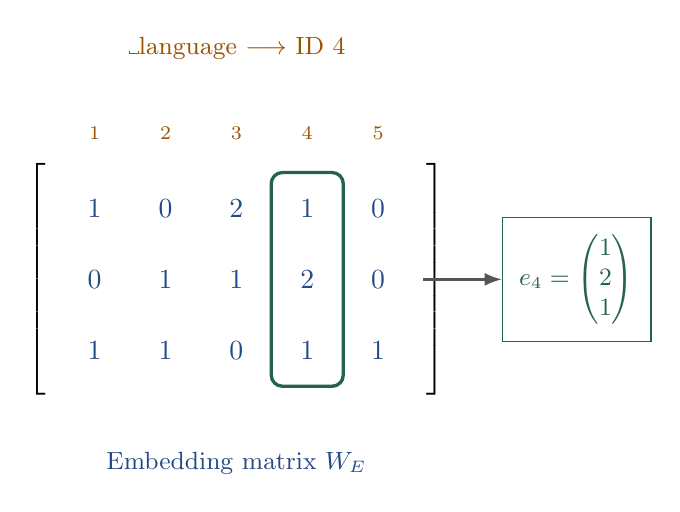
\begin{tikzpicture}
\matrix (m) [matrix of math nodes,nodes={minimum width=9mm,minimum height=9mm,text=Weight},
 left delimiter={[},right delimiter={]}] {1&0&2&1&0\\0&1&1&2&0\\1&1&0&1&1\\};
\foreach \j in {1,2,3,4,5} \node[above=3mm,font=\scriptsize,text=Data] at (m-1-\j.north) {\j};
\draw[Vec,very thick,rounded corners] (m-1-4.north west) rectangle (m-3-4.south east);
\node[above=12mm of m,text=Data,font=\small] {\textvisiblespace language $\longrightarrow$ ID 4};
\node[vector,right=10mm of m] (e) {$e_4=\begin{pmatrix}1\\2\\1\end{pmatrix}$};
\draw[flow] (m.east)--(e.west);
\node[below=6mm of m,text=Weight,font=\small] {Embedding matrix $W_E$};
\end{tikzpicture}
\end{adjustbox}
\end{columns}
\msg{The table is learned during training. A lookup returns the selected column as an \textbf{activation}.}
\src{\cite{sanderson2024} Supplementary toy model: $d=3$, $V=5$. Equivalently, $e_i=W_Eu_i$, where $u_i$ is a one-hot vector.}
\end{frame}

% 15 ---------------------------------------------------------------
\section[Space]{Geometry of meaning}
\begin{frame}[fragile]{Embedding space: proximity can express similarity}
\begin{columns}[T,onlytextwidth]
\column{.56\textwidth}
\centering
\begin{adjustbox}{max width=\linewidth,max totalheight=4.2cm}
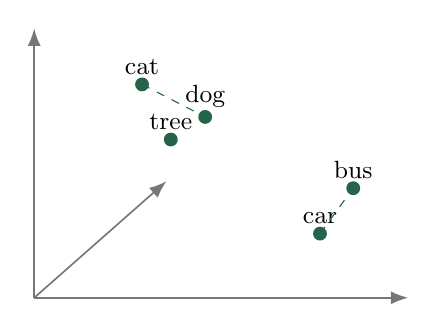
\begin{tikzpicture}[x={(.95cm,0cm)},y={(.42cm,.37cm)},z={(0cm,.9cm)}]
\draw[axis] (0,0,0)--(5,0,0);\draw[axis] (0,0,0)--(0,4,0);\draw[axis] (0,0,0)--(0,0,3.8);
\foreach \x/\y/\z/\s in {1/1/2.6/cat,1.8/1.1/2.1/dog,3.6/.5/.7/car,4/.6/1.3/bus,.5/3/1/tree} {
 \fill[Vec] (\x,\y,\z) circle (2.5pt);
 \node[above,font=\small] at (\x,\y,\z) {\s};}
\draw[Vec,dashed] (1,1,2.6)--(1.8,1.1,2.1);
\draw[Vec,dashed] (3.6,.5,.7)--(4,.6,1.3);
\end{tikzpicture}
\end{adjustbox}
\column{.40\textwidth}
The \textbf{embedding space} is the vector space of token representations.\\[3mm]
\textbf{Semantic similarity}: terms occur with similar meanings or in similar contexts.\\[3mm]
Training can encode these patterns in distances and directions.
\end{columns}
\msg{This is a \textbf{constructed 3D illustration}. Real projections lose information.}
\src{\cite{sanderson2024} Proximity depends on the model and metric. Individual axes need not have an interpretable meaning.}
\end{frame}

% 16 ---------------------------------------------------------------
\begin{frame}[fragile]{Semantic directions: arithmetic with relationships}
\[
\vv{v_{\text{queen}}}\ \approx\ 
\vv{v_{\text{king}}}-\vv{v_{\text{man}}}+\vv{v_{\text{woman}}}
\]
\begin{columns}[T,onlytextwidth]
\column{.56\textwidth}
\centering
\begin{adjustbox}{max width=\linewidth,max totalheight=4.2cm}
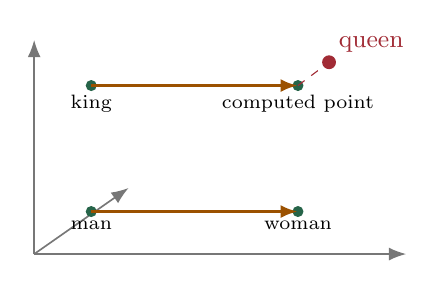
\begin{tikzpicture}[x={(1.05cm,0cm)},y={(.4cm,.28cm)},z={(0cm,.8cm)}]
\draw[axis] (0,0,0)--(4.5,0,0);\draw[axis] (0,0,0)--(0,3,0);\draw[axis] (0,0,0)--(0,0,3.4);
\coordinate (m) at (.5,.5,.5);\coordinate (f) at (3,.5,.5);
\coordinate (k) at (.5,.5,2.5);\coordinate (q) at (3,.5,2.5);
\foreach \p/\s in {m/man,f/woman,k/king,q/{computed point}} {
 \fill[Vec] (\p) circle (2pt);\node[below,font=\scriptsize] at (\p) {\s};}
\draw[->,Data,very thick] (m)--(f);
\draw[->,Data,very thick] (k)--(q);
\fill[Prob] (3.3,.7,2.8) circle (2.5pt);
\node[above right,font=\small,Prob] at (3.3,.7,2.8) {queen};
\draw[dashed,Prob] (q)--(3.3,.7,2.8);
\end{tikzpicture}
\end{adjustbox}
\column{.40\textwidth}
A \textbf{difference vector} is the arrow from one term to another.
\[
\dat{r}=v_{\text{woman}}-v_{\text{man}}
\]
Apply the same displacement to $v_{\text{king}}$ 
\medskip

A similar idea for singular/plural:
\[
\begin{aligned}
v_{\text{cats}}-v_{\text{cat}}\\
\approx v_{\text{dogs}}-v_{\text{dog}}.
\end{aligned}
\]
\end{columns}
\end{frame}

% 17 ---------------------------------------------------------------
\section[Product]{Dot product}
\begin{frame}[fragile]{Dot product: multiply pairs, then add}
\begin{columns}[T,onlytextwidth]
\column{.43\textwidth}
The \textbf{dot product} takes two vectors of the same dimension and returns one number.
\[
a\cdot b=\sum_{i=1}^n a_i b_i
\]
\[
\begin{gathered}
\vv{a=(2,1,0)},\\
\dat{b=(1,3,2)}
\end{gathered}
\]
\[
\begin{aligned}
a\cdot b&=2\cdot1+1\cdot3+0\cdot2\\
&=\pr5.
\end{aligned}
\]
\column{.53\textwidth}
\centering
\begin{adjustbox}{max width=\linewidth,max totalheight=4.2cm}
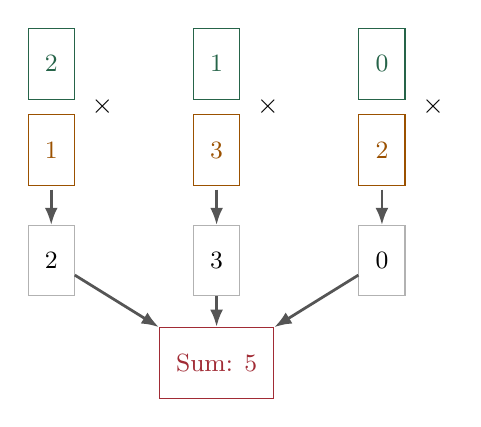
\begin{tikzpicture}
\foreach \x/\a/\b/\r in {0/2/1/2,2.1/1/3/3,4.2/0/2/0} {
 \node[vector] at (\x,1.1) {\a};\node[input] at (\x,0) {\b};
 \node at (\x+.65,.55) {$\times$};
 \node[box] (r\r) at (\x,-1.4) {\r};
 \draw[flow] (\x,-.5)--(\x,-.95);}
\node[output] (s) at (2.1,-2.7) {Sum: 5};
\draw[flow] (r2)--(s);\draw[flow] (r3)--(s);\draw[flow] (r0)--(s);
\end{tikzpicture}
\end{adjustbox}
\end{columns}
\msg{Each row of a matrix-vector product computes a dot product with the input vector.}
\src{\cite{sanderson2024} Supplementary numerical example. The output dimension of $Wx$ equals the number of row-wise dot products.}
\end{frame}

% 18 ---------------------------------------------------------------
\begin{frame}[fragile]{The dot product measures alignment and magnitude}
\[
a\cdot b=\|a\|\,\|b\|\cos\theta
\]
\centering
\begin{adjustbox}{max width=\linewidth,max totalheight=4.2cm}
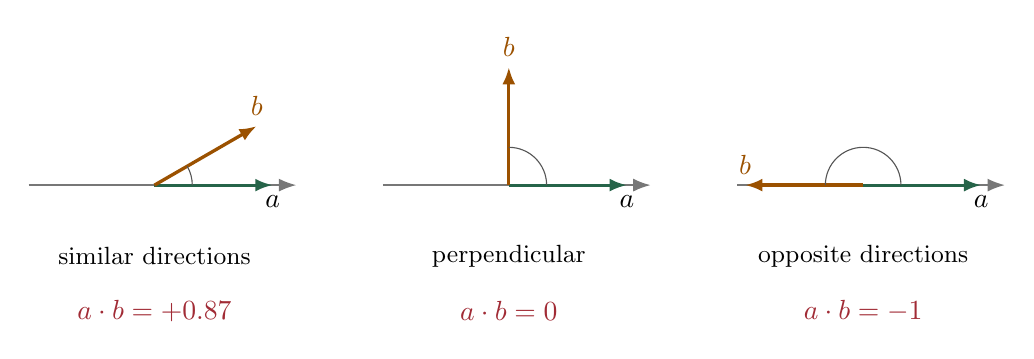
\begin{tikzpicture}
\foreach \x/\ang/\lab/\val in {0/30/{similar directions}/{+0.87},4.5/90/{perpendicular}/{0},9/180/{opposite directions}/{-1}} {
 \begin{scope}[shift={(\x,0)}]
 \draw[axis] (-1.6,0)--(1.8,0);
 \draw[vflow] (0,0)--(1.5,0) node[below]{$a$};
 \draw[->,Data,very thick] (0,0)--(\ang:1.5) node[above]{$b$};
 \draw[Muted] (.48,0) arc[start angle=0,end angle=\ang,radius=.48];
 \node[font=\small] at (0,-.9) {\lab};
 \node[text=Prob] at (0,-1.6) {$a\cdot b=\val$};
 \end{scope}}
\end{tikzpicture}
\end{adjustbox}
\vspace{2mm}
\begin{columns}[T,onlytextwidth]
\column{.48\textwidth}
\small Shown: unit vectors, $\|a\|=\|b\|=1$.\\
In general, \textbf{vector lengths also affect} the result.
\column{.48\textwidth}
\small \textbf{Cosine similarity} isolates direction:\\
$\cos\theta=(a\cdot b)/(\|a\|\|b\|)$ for $a,b\ne0$.
\end{columns}
\src{\cite{sanderson2024} Connection to attention: dot products of learned projections produce compatibility scores.}
\end{frame}

% 19 ---------------------------------------------------------------
\section[Context]{Context}
\begin{frame}[fragile]{Same token -- different representations in context}
\centering
\begin{adjustbox}{max width=\linewidth,max totalheight=4.2cm}
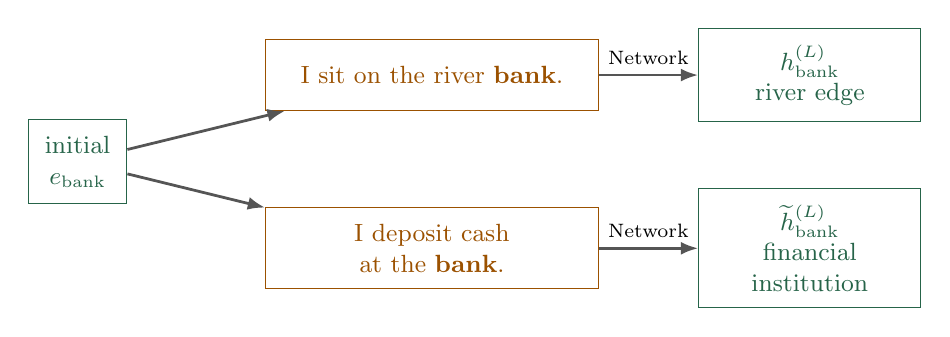
\begin{tikzpicture}
\node[vector] (e) at (0,0) {initial\\$e_{\text{bank}}$};
\node[input,text width=3.8cm] (a) at (4.5,1.1) {I sit on the river \textbf{bank}.};
\node[input,text width=3.8cm] (b) at (4.5,-1.1) {I deposit cash at the \textbf{bank}.};
\node[vector,text width=2.4cm] (c) at (9.3,1.1) {$h_{\text{bank}}^{(L)}$\\river edge};
\node[vector,text width=2.4cm] (d) at (9.3,-1.1) {$\widetilde h_{\text{bank}}^{(L)}$\\financial institution};
\draw[flow] (e)--(a);\draw[flow] (e)--(b);
\draw[flow] (a)--node[above,font=\scriptsize]{Network}(c);
\draw[flow] (b)--node[above,font=\scriptsize]{Network}(d);
\end{tikzpicture}
\end{adjustbox}
\[
\vv{e_i}\ \longrightarrow\ \vv{h_i^{(1)}}\ \longrightarrow\ 
\vv{h_i^{(2)}}\ \longrightarrow\ \vv{h_i^{(L)}}
\]
\msg{A \textbf{contextual vector} represents the token at this position in the text, beyond its dictionary entry.}
\src{\cite{sanderson2024} Constructed example: assume the same token and ID. Position also affects the representation.\\
Context provides clues but does not guarantee the correct interpretation.}
\end{frame}

% 20 ---------------------------------------------------------------
\begin{frame}[fragile]{Context and position: why does order matter?}
\centering
\begin{adjustbox}{max width=\linewidth,max totalheight=4.2cm}
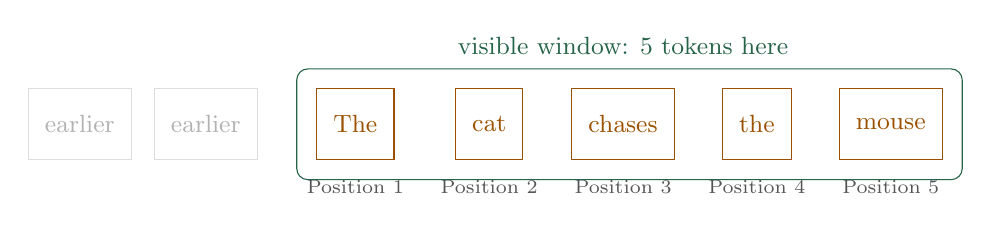
\begin{tikzpicture}
\foreach \x/\s in {0/earlier,1.6/earlier} \node[box,text=Muted!45,draw=Muted!20] at (\x,0) {\s};
\foreach \x/\s/\i in {3.5/The/1,5.2/cat/2,6.9/chases/3,8.6/the/4,10.3/mouse/5} {
 \node[input] (t\i) at (\x,0) {\s};
 \node[tinylabel] at (\x,-.8) {Position \i};}
\node[draw=Vec,rounded corners,fit=(t1)(t5),inner sep=7pt] {};
\node[text=Vec,font=\small] at (6.9,1) {visible window: 5 tokens here};
\end{tikzpicture}
\end{adjustbox}
\begin{columns}[T,onlytextwidth]
\column{.48\textwidth}
\textbf{Context Size}: maximum number of token positions considered. Excluded text is not directly available.
\column{.48\textwidth}
\textbf{Position} distinguishes, for example:\\
``The cat chases the mouse''\ and\\
``The mouse chases the cat''.
\end{columns}
\[
\vv{h_i^{(0)}}=\vv{e_{t_i}}+\w{p_i}
\qquad\text{(example: additive position vectors)}
\]
\src{\cite{sanderson2024,vaswani2017} Supplement: additive positional embeddings are one option, not a universal formula for all Transformers.\\
The diagram shows a simplified window. The application selects which text enters the context.}
\end{frame}

% 21 ---------------------------------------------------------------
\section[Architecture]{Transformer architecture}
\begin{frame}[fragile]{The complete data flow of a GPT language model}
\centering
\begin{adjustbox}{max width=\linewidth,max totalheight=4.2cm}
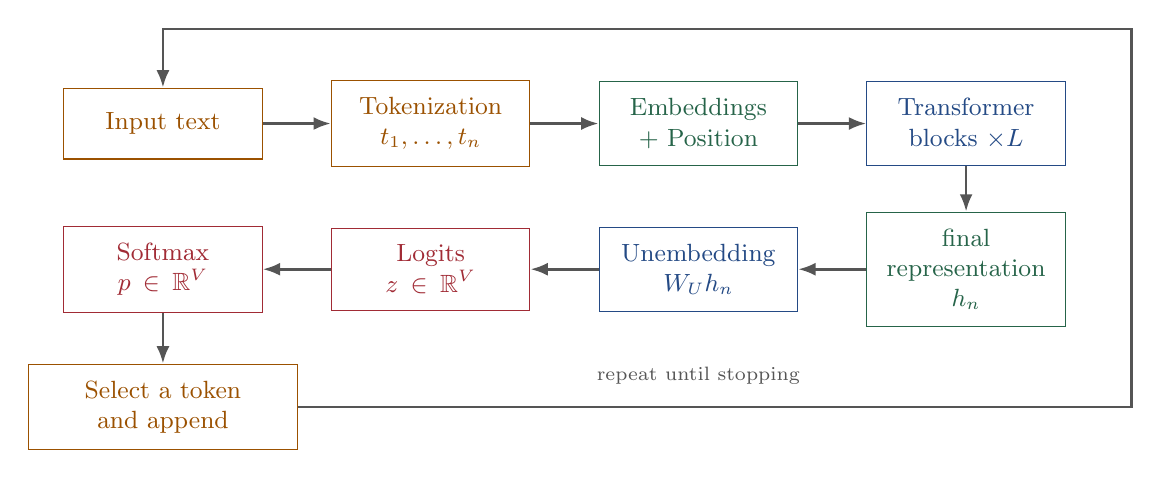
\begin{tikzpicture}
\node[input,text width=2.1cm] (a) at (0,0) {Input text};
\node[input,text width=2.1cm] (b) at (3.4,0) {Tokenization\\$t_1,\ldots,t_n$};
\node[vector,text width=2.1cm] (c) at (6.8,0) {Embeddings\\+ Position};
\node[param,text width=2.1cm] (d) at (10.2,0) {Transformer\\blocks $\times L$};
\node[vector,text width=2.1cm] (e) at (10.2,-1.85) {final\\representation $h_n$};
\node[param,text width=2.1cm] (f) at (6.8,-1.85) {Unembedding\\$W_Uh_n$};
\node[output,text width=2.1cm] (g) at (3.4,-1.85) {Logits\\$z\in\R^V$};
\node[output,text width=2.1cm] (h) at (0,-1.85) {Softmax\\$p\in\R^V$};
\node[input,text width=3cm] (i) at (0,-3.6) {Select a token\\and append};
\draw[flow] (a)--(b);\draw[flow] (b)--(c);\draw[flow] (c)--(d);
\draw[flow] (d)--(e);\draw[flow] (e)--(f);\draw[flow] (f)--(g);\draw[flow] (g)--(h);
\draw[flow] (h)--(i);
\draw[flow] (i.east)--(12.3,-3.6)--(12.3,1.2)--(0,1.2)--(a.north);
\node[tinylabel] at (6.8,-3.2) {repeat until stopping};
\end{tikzpicture}
\end{adjustbox}
\src{\cite{sanderson2024} Schematic GPT architecture. The representation at the last position $n$ predicts the next token.\\
Colours: orange = tokens; blue = parameters; green = representations; red = scores and probabilities.}
\end{frame}

% 22 ---------------------------------------------------------------
\begin{frame}[fragile]{Two recurring tasks inside a Transformer block}
\begin{columns}[T,onlytextwidth]
\column{.54\textwidth}
\centering
\begin{adjustbox}{max width=\linewidth,max totalheight=4.2cm}
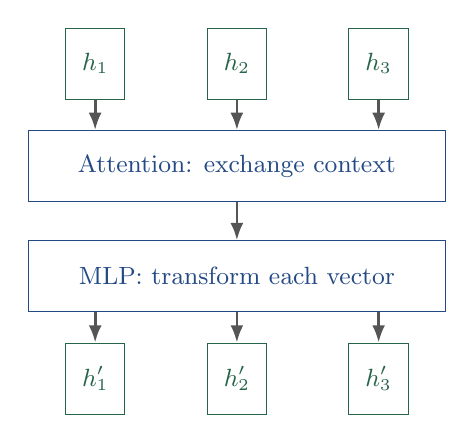
\begin{tikzpicture}
\foreach \x/\i in {0/1,1.8/2,3.6/3} \node[vector] (e\i) at (\x,0) {$h_{\i}$};
\node[param,minimum width=5.3cm] (a) at (1.8,-1.3) {Attention: exchange context};
\node[param,minimum width=5.3cm] (m) at (1.8,-2.7) {MLP: transform each vector};
\foreach \i in {1,2,3} \draw[flow] (e\i)--(a.north-|e\i);
\draw[flow] (a)--(m);
\foreach \x/\i in {0/1,1.8/2,3.6/3} {
 \node[vector] (o\i) at (\x,-4) {$h'_{\i}$};
 \draw[flow] (m.south-|o\i)--(o\i);}
\end{tikzpicture}
\end{adjustbox}
\column{.42\textwidth}
\textbf{Attention}: incorporate relevant earlier positions or the current position.\\[3mm]
\textbf{MLP}, multilayer perceptron: apply the same nonlinear transformation to each position, without direct exchange between positions.\\[3mm]
Repeated blocks produce increasingly contextual representations.
\end{columns}
\src{Supplement: GPT uses causal masking to prevent access to future tokens. Residual connections and normalization are omitted for clarity.}
\end{frame}

% 23 ---------------------------------------------------------------
\begin{frame}[fragile]{From toy examples to the scale of GPT-3}
\begin{columns}[T,onlytextwidth]
\column{.52\textwidth}
\centering
\begin{adjustbox}{max width=\linewidth,max totalheight=4.2cm}
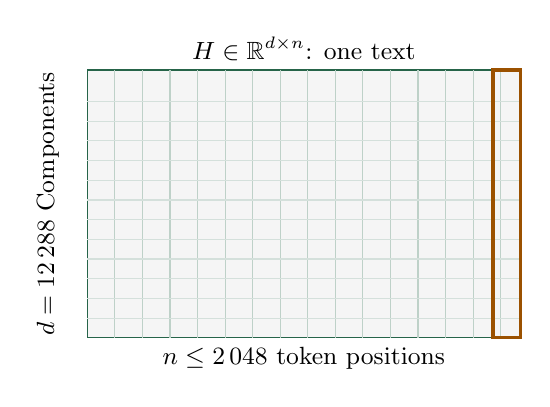
\begin{tikzpicture}
\draw[Vec,fill=Panel] (0,0) rectangle (5.5,3.4);
\foreach \x in {.35,.7,...,5.3} \draw[Vec!30] (\x,0)--(\x,3.4);
\foreach \y in {.25,.5,...,3.2} \draw[Vec!20] (0,\y)--(5.5,\y);
\draw[Data,very thick] (5.15,0) rectangle (5.5,3.4);
\node[above,font=\small] at (2.75,3.4) {$H\in\R^{d\times n}$: one text};
\node[below,font=\small] at (2.75,0) {$n\leq 2\,048$ token positions};
\node[rotate=90,font=\small] at (-.5,1.7) {$d=12\,288$ Components};
\end{tikzpicture}
\end{adjustbox}
\column{.44\textwidth}
\textbf{Historical example: GPT-3 (175B)}
\medskip

Vocabulary: $V=50\,257$ Tokens.\\
Vector dimension: $d=12\,288$.\\
Context: $2\,048$ Tokens.\\
Total: about $175$ billion parameters.
\[
\begin{gathered}
\underbrace{50\,257\cdot12\,288}_{\text{Entries in }W_E}\\
=617\,558\,016
\end{gathered}
\]
\end{columns}
\msg{\textbf{Parameters} are learned tables. The \textbf{activations} in $H$ depend on the input text.}
\src{Supplement: embedding and unembedding can share weights; matching shapes need not imply extra independent parameters.}
\end{frame}

% 24 ---------------------------------------------------------------
\section[Output]{Unembedding}
\begin{frame}[fragile]{Unembedding: one score for each possible token}
\[
\pr{z}=\w{W_U}\vv{h},\qquad
\underbrace{\pr{\begin{pmatrix}2\\1\\0\end{pmatrix}}}_{\text{Logits}}
=\underbrace{\w{\begin{pmatrix}1&0\\0&1\\0&0\end{pmatrix}}}_{3\times2}
\underbrace{\vv{\begin{pmatrix}2\\1\end{pmatrix}}}_{\text{last representation}}
\]
\begin{columns}[T,onlytextwidth]
\column{.49\textwidth}
\textbf{$h$}: final contextual vector at the last input position.\\[2mm]
\textbf{$W_U\in\R^{V\times d}$}: one row per vocabulary entry.\\[2mm]
\textbf{Logits}: unnormalized scores, not yet probabilities.
\column{.46\textwidth}
\centering
\begin{adjustbox}{max width=\linewidth,max totalheight=4.2cm}
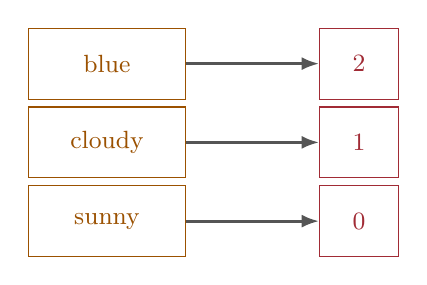
\begin{tikzpicture}
\foreach \y/\s/\l in {0/blue/2,-1/cloudy/1,-2/sunny/0} {
 \node[input,minimum width=2cm] (t\l) at (0,\y) {\s};
 \node[output,minimum width=1cm] (z\l) at (3.2,\y) {\l};
 \draw[flow] (t\l)--(z\l);}
\end{tikzpicture}
\end{adjustbox}
\end{columns}
\end{frame}

% 25 ---------------------------------------------------------------
\section[Softmax]{Softmax and temperature}
\begin{frame}[fragile]{Softmax: make scores positive, then normalize}
\[
\pr{p_i}=\frac{e^{z_i}}{\sum_j e^{z_j}}
\]
\centering
\begin{adjustbox}{max width=\linewidth,max totalheight=4.2cm}
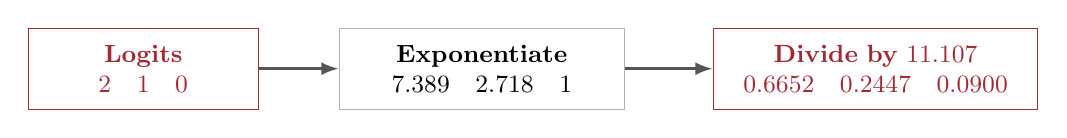
\begin{tikzpicture}
\node[output,text width=2.5cm] (z) at (0,0) {\textbf{Logits}\\$2\quad1\quad0$};
\node[box,text width=3.2cm] (e) at (4.3,0) {\textbf{Exponentiate}\\$7.389\quad2.718\quad1$};
\node[output,text width=3.7cm] (p) at (9.3,0) {\textbf{Divide by $11.107$}\\$0.6652\quad0.2447\quad0.0900$};
\draw[flow] (z)--(e);\draw[flow] (e)--(p);
\end{tikzpicture}
\end{adjustbox}
\vspace{3mm}
\begin{columns}[T,onlytextwidth]
\column{.53\textwidth}
\small
\textbf{Why $e^z$?} Always positive, strictly increasing and smooth. Score differences become ratios:
\[
\begin{gathered}
\frac{p_i}{p_j}=e^{z_i-z_j},\\[2mm]
\sum_i p_i=\frac{\sum_i e^{z_i}}{\sum_j e^{z_j}}=1.
\end{gathered}
\]
This is a suitable choice, though other normalizations are possible.
\column{.43\textwidth}
\centering
\begin{adjustbox}{max width=\linewidth,max totalheight=4.2cm}
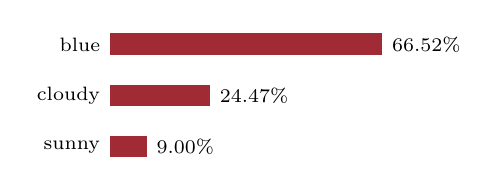
\begin{tikzpicture}[x=.052cm,y=.65cm]
\foreach \y/\v/\s in {2/66.52/blue,1/24.47/cloudy,0/9.00/sunny} {
 \node[left,font=\scriptsize] at (0,\y+.2) {\s};
 \fill[Prob] (0,\y) rectangle (\v,\y+.42);
 \node[right,font=\scriptsize] at (\v,\y+.2) {\v\%};}
\end{tikzpicture}
\end{adjustbox}
\end{columns}
\end{frame}

% 26 ---------------------------------------------------------------
\begin{frame}[fragile]{Temperature controls the concentration of the distribution}
\[
\pr{p_i(T)}=\frac{e^{z_i/T}}{\sum_j e^{z_j/T}},\qquad T>0,
\qquad z=(2,1,0)
\]
\centering
\begin{columns}[T,onlytextwidth]
\column{.32\textwidth}\centering
\bars{$T=0.5$}{86.7}{11.7}{1.6}\par
\small\textbf{Low:} more concentrated, less diverse.
\column{.32\textwidth}\centering
\bars{$T=1$}{66.5}{24.5}{9.0}\par
\small\textbf{One:} original softmax distribution.
\column{.32\textwidth}\centering
\bars{$T=2$}{50.6}{30.7}{18.6}\par
\small\textbf{High:} flatter distribution, more randomness.
\end{columns}
\end{frame}

% 27 ---------------------------------------------------------------
\begin{frame}[fragile]{Putting it together: training and generation}
\centering
\begin{adjustbox}{max width=\linewidth,max totalheight=4.2cm}
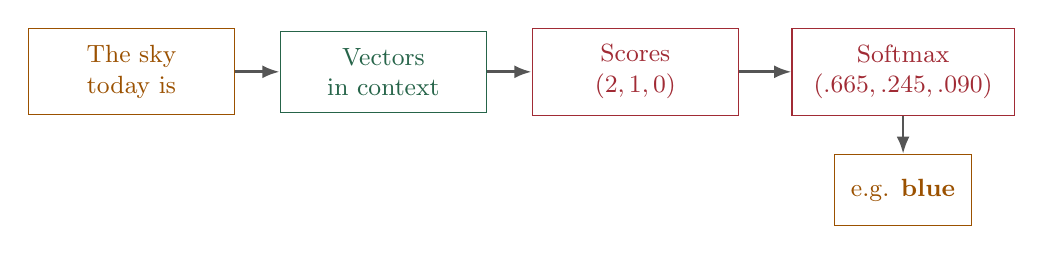
\begin{tikzpicture}
\node[input,text width=2.2cm] (a) at (0,0) {The sky\\today is};
\node[vector,text width=2.2cm] (b) at (3.2,0) {Vectors\\in context};
\node[output,text width=2.2cm] (c) at (6.4,0) {Scores\\$(2,1,0)$};
\node[output,text width=2.4cm] (d) at (9.8,0) {Softmax\\$(.665,.245,.090)$};
\draw[flow] (a)--(b);\draw[flow] (b)--(c);\draw[flow] (c)--(d);
\node[input] (s) at (9.8,-1.5) {e.g. \textbf{blue}};\draw[flow] (d)--(s);
\end{tikzpicture}
\end{adjustbox}
\vspace{3mm}
\begin{columns}[T,onlytextwidth]
\column{.48\textwidth}
\textbf{Training changes weights.}\\
The actual next token is the target; a low target probability incurs a higher loss:
\[
\begin{gathered}
L=-\log p(\text{target token}),\\
-\log(0.6652)\approx0.408.
\end{gathered}
\]
\column{.48\textwidth}
\textbf{Generation changes the text.}\\
During standard inference, weights stay fixed. Sample a token, append it and process the updated context.\\[2mm]
\textbf{Key idea:} Tokens become vectors, context transforms vectors, and scores become probabilities.
\end{columns}
\src{\cite{sanderson2024} Supplement: simplified training loss using the natural logarithm; averaged over many positions.\\
During training, many next-token predictions can be computed in parallel; causal masking hides their target tokens.}
\end{frame}

% 28 ---------------------------------------------------------------
\section[References]{References}
\begin{frame}{References}
\small
\begin{thebibliography}{9}
\setlength{\itemsep}{.7em}
\bibitem{sanderson2024}
Sanderson, G. (3Blue1Brown) (2024).
\newblock \emph{Transformers, the tech behind LLMs -- Deep Learning Chapter 5}.
\newblock Video, 1 April 2024.
\href{https://youtu.be/wjZofJX0v4M}{youtu.be/wjZofJX0v4M}.\\
\href{https://www.3blue1brown.com/lessons/gpt/}{Companion article: 3blue1brown.com/lessons/gpt/}.

\bibitem{vaswani2017}
Vaswani, A., et al. (2017).
\newblock \emph{Attention Is All You Need}.
\newblock arXiv:1706.03762.
\href{https://doi.org/10.48550/arXiv.1706.03762}{doi:10.48550/arXiv.1706.03762}.

\bibitem{brown2020}
Brown, T. B., et al. (2020).
\newblock \emph{Language Models are Few-Shot Learners}.
\newblock arXiv:2005.14165.
\href{https://doi.org/10.48550/arXiv.2005.14165}{doi:10.48550/arXiv.2005.14165}.
\end{thebibliography}
\medskip
{\scriptsize Online sources accessed 17 November 2026.
Diagrams and explicitly marked numerical examples: own illustrations.}
\end{frame}
\end{document}
